\documentclass{article}

\usepackage[top=1in,left=1.5in,right=1.5in,bottom=1.5in]{geometry}

\usepackage{subcaption}

\usepackage{booktabs}

\usepackage{graphicx}
\let\rfb\reflectbox
\graphicspath{ {images} }
 
\usepackage{mathtools}

\usepackage{nicefrac}
\newcommand{\flippedfrac}[2]{\rfb{\nicefrac{\rfb{#2}}{\rfb{#1}}}}



\usepackage{amsthm}
\renewcommand{\qedsymbol}{$\blacksquare$}
\usepackage{amssymb}
\usepackage{amsmath}
\newcommand\numberthis{\addtocounter{equation}{1}\tag{\theequation}}

\usepackage{hyperref}
\hypersetup{
    colorlinks = true,
}


\usepackage{titling}
\title{Exercise Set 2 - Reinforcement Learning}
\newcommand{\subtitle}[1]{%
  \posttitle{%
    \par\end{center}
    \begin{center}\large#1\end{center}
    \vskip0.5em}%
}
\makeatother
\subtitle{Tabular Methods}
\author{Giulio Starace - 13010840}
\date{\today}

\begin{document}
\maketitle
\section*{Homework: Coding Assignment - Monte Carlo}
\begin{enumerate}
	\item To derive the incremental update rule of the value function for a given state $V(s)$ using
	      ordinary importance sampling, we begin with the definition of the estimate $V_n(s)$ given $n$
	      sampled returns $G_1, \dots, G_n$ under this regime:
	      \begin{equation}\label{eq:value_function_estimate}
		      V_n(s) = \frac{1}{n} \sum^n_{k=1} W_k G_k,
	      \end{equation}
	      where $W_k$ is the importance sampling ratio of target policy $\pi$ over behavior policy $b$.
	      \begin{equation}
		      W_k = \rho_{t_k:T(t_k)-1} = \prod_{t=t_k}^{T(t_k)-1} \frac{\pi(A_t|S_t)}{b(A_t|S_t)}.
	      \end{equation}
	      We expand equation (\ref{eq:value_function_estimate}) to obtain:
	      \begin{align*}
		      V_n(s) & = \frac{1}{n} \left[W_{n-1} G_{n-1} + \sum^{n-1}_{i=1}W_kG_k\right]                \\
		             & = \frac{1}{n} \left[W_{n-1} G_{n-1} +
		      (n-1)\underbracket{\left(\frac{1}{n-1}\right)\sum^{n-1}_{i=1}W_kG_k}\right]                 \\
		             & =  \frac{1}{n} \left[W_{n-1} G_{n-1}+ (n-1)\underbracket{V_{n-1}(s)} \right]       \\
		             & = \frac{1}{n} \left[W_{n-1} G_{n-1}+ n V_{n-1}(s) - V_{n-1}(s)\right]              \\
		      V_n(s) & =  V_{n-1}(s) + \frac{1}{n} \left[W_{n-1} G_{n-1} - V_{n-1}(s)\right]. \numberthis
		      \label{eq:incremental_update_rule}
	      \end{align*}
	      We see that equation (\ref{eq:incremental_update_rule}) is of the form
	      \begin{equation}
		      V_n = V_{n-1} + \alpha * \left(\beta - V_{n-1}\right),
	      \end{equation}
	      with $\alpha = \frac{1}{n}$ and $\beta = W_{n-1} G_{n-1}$.  \\ \qed

	\item Coding answers have been submitted on codegra under the group ``stalwart cocky sawly".
	      Please refer to Figures \ref{fig:figure_5.1} and \ref{fig:v_function} for the requested figures.
	      \begin{figure}[ht]
		      \centering
		      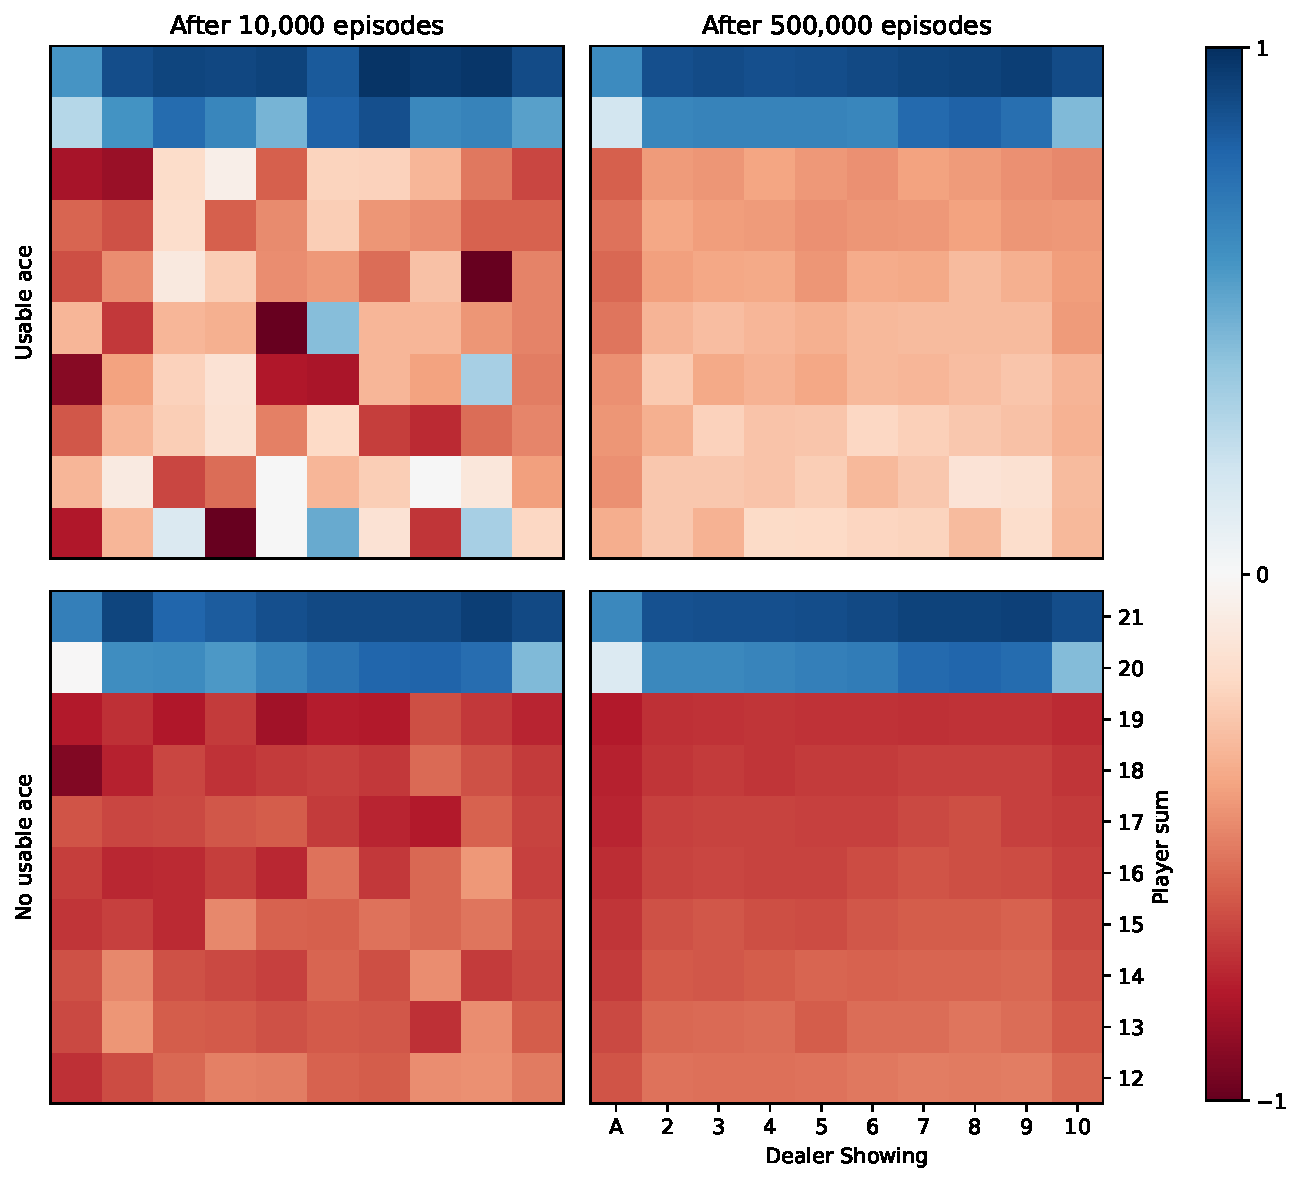
\includegraphics[width=\textwidth]{fig_5.1}
		      \caption{Blackjack value function across state configurations after 10k and 500k episodes
			      using on-policy MC prediction. Reproduction of figure 5.1 from Sutton and Barto, using
			      heatmaps.}
		      \label{fig:figure_5.1}
	      \end{figure}

	      \begin{figure}[ht]
		      \centering
		      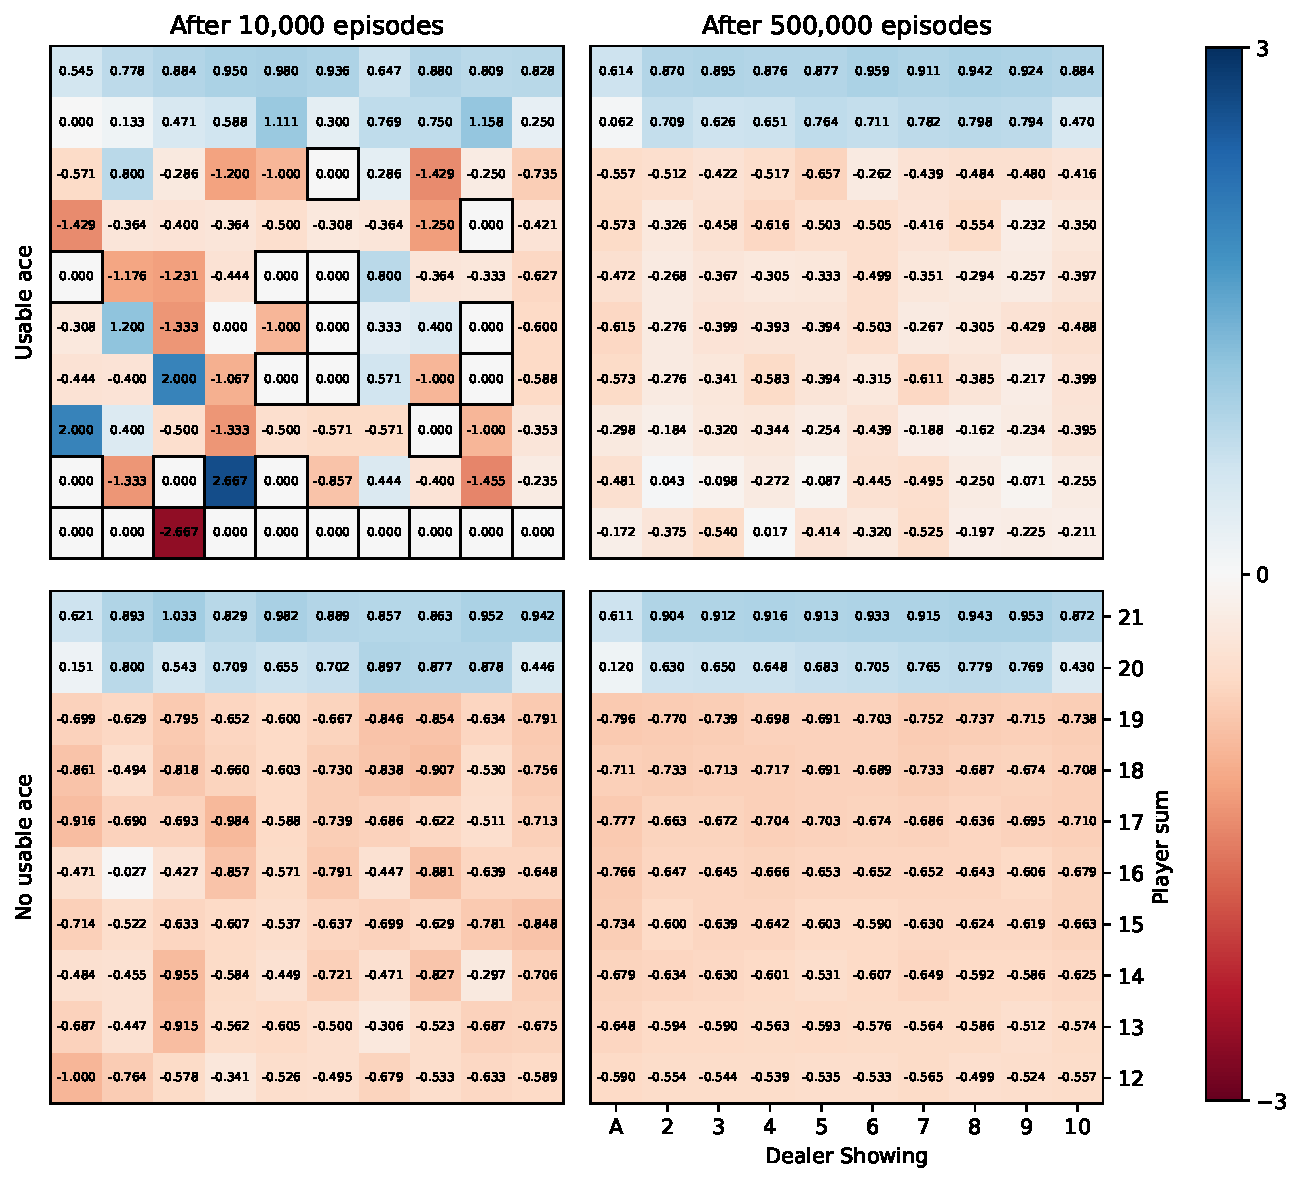
\includegraphics[width=\textwidth]{fig_5.1_off_policy}
		      \caption{Blackjack value function across state configurations after 10k and 500k episodes
			      using off-policy MC prediction with ordinary importance sampling.}
		      \label{fig:v_function}
	      \end{figure}
	\item The main difference between Dynamic Programming (DP) and Monte Carlo (MC) is that the former assumes
	      a perfect model (complete knowledge) of the environment, while the latter does not, relying
	      on experience instead. Furthermore, unlike DP methods, MC methods do not \textit{bootstrap},
	      i.e. they do not update their estimates using other estimates. MC methods are better suited
	      in situations where the environment is not known and needs to be learned about. DP on the
	      other hand is better suited in situations where the environment is known and we can afford
	      to compute the value function of each state.

\end{enumerate}

\section*{Homework: SARSA and Q-learning}
\begin{enumerate}
	\item \begin{enumerate}
		      \item Please refer to Table \ref{tab:converged_sarsa} for the final Q-values for all
		            states and actions after converging un-discounted SARSA with an $\epsilon$-greedy
		            policy with $\epsilon=0.1$.
		      \item The final policy will prefer to choose action $a_1$ more often in state A when $Q(A,
			            a_1) > Q(A, a_0)$, that is when
		            \begin{align*}
			            Q(A,a_1)    & > Q(A, a_0) \\
			            3.9 + 0.05n & > 2         \\
			            n           & > -38
		            \end{align*}
		            i.e when $n \in (-38, 2)$. Similarly the final policy will prefer to choose action
		            $a_0$ more often in state A when $Q(A,
			            a_1) < Q(A, a_0)$, that is when
		            \begin{align*}
			            Q(A,a_1)    & < Q(A, a_0) \\
			            3.9 + 0.05n & < 2         \\
			            n           & < -38
		            \end{align*}
		            i.e when $n \in (-\infty, -38)$. When $n = 38$, the final policy will choose between
		            actions $a_0$ and $a_1$ arbitrarily.
	      \end{enumerate}
	\item \begin{enumerate}
		      \item Please refer to Table \ref{tab:converged_qlearning} for the final Q-values for all
		            states and actions after converging un-discounted Q-learning.
		      \item The final policy will prefer to choose action $a_1$ more often in state A when $Q(A,
			            a_1) > Q(A, a_0)$, that is when
		            \begin{align*}
			            Q(A,a_1)       & > Q(A, a_0) \\
			            2 + \max(2, n) & > 2         \\
			            \max(2,n)      & > 0
		            \end{align*}
		            This condition remains true regardless of the value of $n$, so the final policy will
		            always prefer to choose action $a_1$ when in state $A$, for any $n \in (-\infty,
			            \infty)$. As such, the final policy will never choose $a_0$ in state $A$, i.e. for
		            none of the values of $n$.
		            \begin{table}[h]
			            \caption{Converged Q-values for SARSA and Q-learning, assuming
				            initialization at 0.}
			            \begin{subtable}{0.5\linewidth}\centering
				            \begin{tabular}{@{}ccccc@{}}
					            \toprule
					                  & A             & B & C   & T \\ \midrule
					            $a_0$ & 2             & 1 & 2   & 0 \\
					            $a_1$ & $3.9 + 0.05n$ & 0 & $n$ & 0 \\ \bottomrule
				            \end{tabular}
				            \caption{Q-values for all states and actions at SARSA convergence.}
				            \label{tab:converged_sarsa}
			            \end{subtable}
			            \quad
			            \begin{subtable}{0.5\linewidth}\centering
				            \begin{tabular}{@{}ccccc@{}}
					            \toprule
					                  & A                & B & C   & T \\ \midrule
					            $a_0$ & 2                & 1 & 2   & 0 \\
					            $a_1$ & $2 + \max(2, n)$ & 0 & $n$ & 0 \\ \bottomrule
				            \end{tabular}
				            \caption{Q-values for all states and actions at Q-learning convergence.}
				            \label{tab:converged_qlearning}
			            \end{subtable}
			            \label{tab:converged}
		            \end{table}
	      \end{enumerate}
	\item With $n=1$ and the addition of an extra action $a_2$ in $A$ causing a transition to
	      $B$ with reward 1, the final performance (average return after convergence) of Q-learning would
	      remain the same. This is because Q-learning converges to the optimal policy, choosing the action
	      with the maximum value, which in this case, remains to be $a_1$, as $a_2$ provides the same
	      effect as $a_0$, which we have established is never chosen by a converged Q-learning policy.
	      The final performance of SARSA on the other hand would decrease, as there are now more
	      actions to choose from in state $A$, causing the policy to choose greedily less often.
\end{enumerate}


\end{document}
